\part*{TEMPORARY - CM4}

\section{The divide and conquer principle (end) and dynamic programing}

    \subsection{Divide and conquer : \texttt{DeterministicSelect(T,i)}}



In the previous course, we determine the \texttt{RandomSelect(T,i)} algorithm in which we can find the $i^{th}$ smallest entry of an array T in $\Theta (n)$ (worst-case expected time). This algorithm was based on a variance of the quick sort.

The question asked is : Can we do it deterministic O(n) time?

To answer it, we must find a good pivot deterministically. This lead us to the following \texttt{DeterministicSelect(T,i)} (List.\ref{list:c4:deterministicselect}).

\begin{lstlisting}[label={list:c4:deterministicselect},caption=Pseudo-code of the DeterminisicSelect algorithm]
DeterministicSelect(T,i) :
    Split T into ceiling(n/5) arrays of maxsize = 5 
    
    foreach array : 
        find median % ceiling(n/5) medians = Theta(ceiling(n/5))
        
    Pivot = DeterminisiticSelect(medians, 1/2 * ceiling(n/5)) 
        % find the median of the medians computed
    
    Tlow = entries < pivot
    Thight = entries > pivot
    
    if (i <= |Tlow|)
        return DeterministicSelect(Tlow,i)
    if (i == |Tlow| + 1) 
        return pivot
    if (i > |Tlow| + 1)
        return DeterministicSelect(Thigh,i-|Tlow|-1)
\end{lstlisting}



Is this a good pivot?

As our pivot is the median of the different medians, we can say for sure that for the half of the array, the pivot is higher than the 3 smallest values (the median and the values smaller than the median). Thus we can affirm that the pivot is higher than at least $3\times \frac{1}{2} \times \ceil{\frac{n}{5}} \approx \frac{3n}{10}$.

We can do the same reasoning for the value higher than the pivot and also affirm that at least $3\times \frac{1}{2} \times \ceil{\frac{n}{5}} \approx \frac{3n}{10}$ values are higher for sure.

A simple drawing (Fig.\ref{fig:c4:deterministicselect}) can easily illustrate this reasoning.

\begin{figure}
\centering
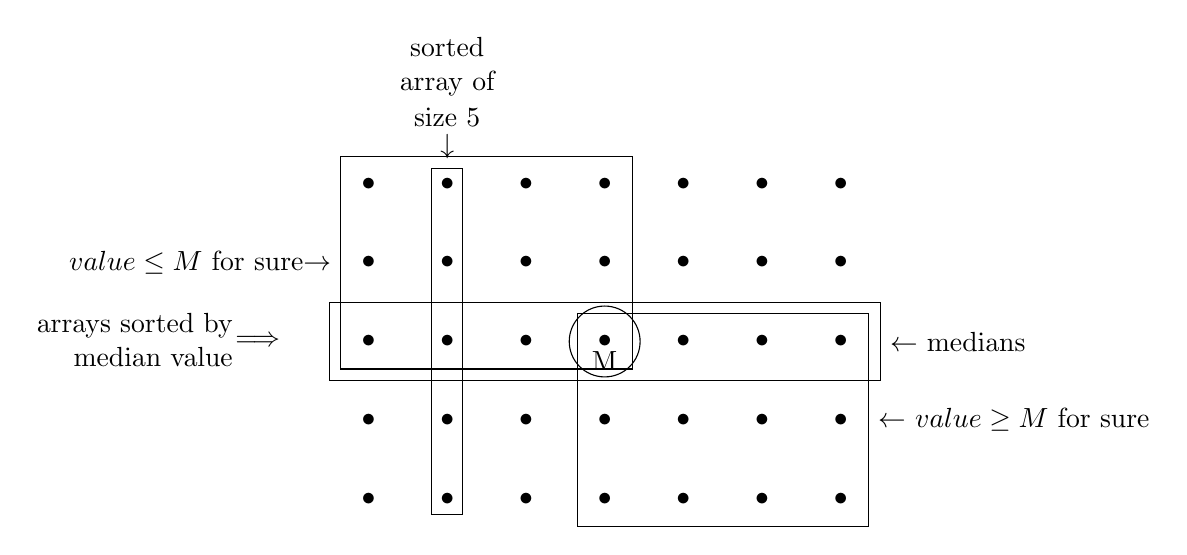
\begin{tikzpicture}
\draw (0,0) node {$\bullet$} ;
\draw (0,1) node {$\bullet$} ;
\draw (0,2) node {$\bullet$} ;
\draw (0,3) node {$\bullet$} ;
\draw (0,4) node {$\bullet$} ;
\draw (1,0) node {$\bullet$} ;
\draw (1,1) node {$\bullet$} ;
\draw (1,2) node {$\bullet$} ;
\draw (1,3) node {$\bullet$} ;
\draw (1,4) node {$\bullet$} ;
\draw (2,0) node {$\bullet$} ;
\draw (2,1) node {$\bullet$} ;
\draw (2,2) node {$\bullet$} ;
\draw (2,3) node {$\bullet$} ;
\draw (2,4) node {$\bullet$} ;
\draw (3,0) node {$\bullet$} ;
\draw (3,1) node {$\bullet$} ;
\draw (3,2) node {$\bullet$} ;
\draw (3,3) node {$\bullet$} ;
\draw (3,4) node {$\bullet$} ;
\draw (4,0) node {$\bullet$} ;
\draw (4,1) node {$\bullet$} ;
\draw (4,2) node {$\bullet$} ;
\draw (4,3) node {$\bullet$} ;
\draw (4,4) node {$\bullet$} ;
\draw (5,0) node {$\bullet$} ;
\draw (5,1) node {$\bullet$} ;
\draw (5,2) node {$\bullet$} ;
\draw (5,3) node {$\bullet$} ;
\draw (5,4) node {$\bullet$} ;
\draw (6,0) node {$\bullet$} ;
\draw (6,1) node {$\bullet$} ;
\draw (6,2) node {$\bullet$} ;
\draw (6,3) node {$\bullet$} ;
\draw (6,4) node {$\bullet$} ;
\draw (-1.6,2.2) node[left] {arrays sorted by};
\draw (-1.6,1.8) node[left] {median value};
\draw (-1,2) node[left] {$\Longrightarrow$};
\draw (0.8,-0.2) rectangle (1.2,4.2);
\draw (1,5.5) node[above]{sorted};
\draw (1,5) node[above]{array of};
\draw (1,4.6) node[above]{size 5};
\draw (1,4.2) node[above]{$\downarrow$};
\draw (-0.5,1.5) rectangle (6.5,2.5);
\draw (6.5,2) node[right]{$\leftarrow$ medians} ;
\draw (-0.35,4.35) rectangle (3.35,1.65);
\draw (-0.35,3) node[left]{$value \leq M$ for sure$\rightarrow$};
\draw (2.65,2.35) rectangle (6.35,-0.35);
\draw (6.35,1) node[right]{$\leftarrow$ $value \geq M$ for sure};
\draw (3,2) circle (0.45) ;
\draw (3,2) node[below]{M};
\end{tikzpicture}
\caption{Graphical view of the selection of the pivot (point M) in the \texttt{DeterministiSelect(T,i)}}
\label{fig:c4:deterministicselect}
\end{figure}

Knowing that, we can now compute the complexity of this algorithm by first writing down the recurrence equation :

\begin{align*}
t_n &= \underbrace{\Theta (n)}_{\text{split \& median finding}} + \underbrace{t_{\ent{n/5}}}_{\text{median of median}} + \underbrace{\Theta (n)}_{\text{split high low}} + \underbrace{\max \{ t_{|T_{low}|},1,t_{|T_{high}|} \}}_{\text{if cases}}\\ 
&\leq t_{n/5} + t_{7n/10} + \underbrace{\Theta (n)}_{f(n)}
\end{align*}

\begin{theorem}
$t_n = \mathcal{O} (n)$
\end{theorem}

\paragraph*{Proof.}This will be proven by induction. By the hypothesis $f(n) = \Theta (n)$, we know that $f(n) \leq an$ (with $a>0$) for large enough $n$.

To be $\mathcal{O}(n)$, there must exist $c>0$ such as $t_n \leq cn$.

For $n$ small, the theorem is proven.

Now let's assume it is proven for $1,...,n-1$ and prove it for $n$ :

\begin{align*}
t_n &\leq t_{\frac{n}{5}} + t_{\frac{7n}{10}} + an\\
&\leq c \frac{n}{5} + c \frac{7n}{10} + an \\
&= c \frac{9n}{10} + an\\
&\leq cn &\text{if } a\leq \frac{1}{10}c
\end{align*}
\QED
